\documentclass[a4paper,twoside]{article}
\usepackage{graphicx} % para da cor
\usepackage[brazil]{babel} % Para traduzir nomes que aparecem em inglês na estrutura do documento.
\usepackage[utf8]{inputenc} % This package allows the user to specify an input encoding
\usepackage[T1]{fontenc} % Permite que o LaTeX compreenda a acentuação feita direto pelo teclado. 
\usepackage{amsfonts} % Define alguns estilos de letras para o ambiente matemático
\usepackage{fancyhdr} % Para fazer cabeçalhos personalizados
\usepackage{float}
\usepackage{hyperref} % Para tornar os links clicáveis
\hypersetup{
    colorlinks=true,
    linkcolor=blue,
    filecolor=blue,
    citecolor=blue,
    urlcolor=blue,
}
\usepackage{microtype} % evitando ligatures do tipo ff
\DisableLigatures{encoding = *, family = * }
\title{\textbf{Manifesto Hotmart V2.0.0}}
\author{Vitor Lopes \\ vitor.lopes@hotmart.com}
\begin{document}
\maketitle
\begin{abstract}
    A Hotmart é de longe uma das empresas mais legais de se frequentar, de se fazer novas amizades, de interagir e trocar conhecimento. Tanto é que tudo que foi descrito está presente em seus pilares e mantras presentes nem seu código de conduto. Porém, contudo, entretanto, nem tudo são flores, principalmente no que se diz respeito aos processos e sistemas legais bem como as regras de negócios que ficam por tantas vezes ocultas onde temos que despender tanto tempo para depurá-las.
    Este material tem como objetivo trazer argumentos e propor uma metodologia ágil e divertida para subirmos mais um patamar no desenvolvimento da empresa como um todo.
\end{abstract}
\section{Introdução}
Software legado em alguns contextos pode ser tido como um software de tecnologia obsoleta, mas gostaria de de estender este conceito para todo aquele software, mesmo que tenha acabado de sair do forno, que não desempenha suas funções em sua plenitude e por isso deve ser melhorado ou substituído. Ou seja, é aquele software que veio e uma hora ou outra vai lhe gerar algum tipo de problema. 

Mas então por que softwares legados existem? A resposta é simples: porque ninguém nasce sabendo aonde quer ir. Acompanhe comigo a seguinte situação: uma empresa nasce e começa a ter que fazer suas escolhas. Ao longo do seu caminho, ela opta por boas ou não tão boas assim. Mas quando chega a determinado momento, as escolhas pregressas ajudam que esta empresa comece e ir em um caminho mais coeso. Isso se chama Maturidade.

\begin{figure}[H]
    \centering
    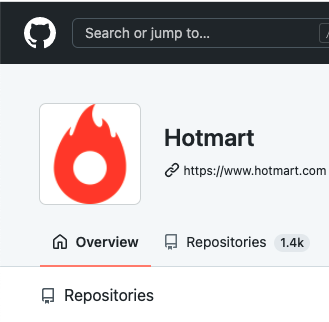
\includegraphics[scale=0.60,keepaspectratio=true]{images/01.png}
    \caption{Processo de amadurecimento}
    \label{mature_process}
\end{figure}

Agora pense, se fosse possível pegarmos tudo de bom e ruim, juntássemos as melhores escolhas desde o momento em que nascemos até o momento em que amadurecemos, seria perfeito. E é exatamente o que é possível fazer com um software: a consolidação do conhecimento. 

\begin{figure}[H]
    \centering
    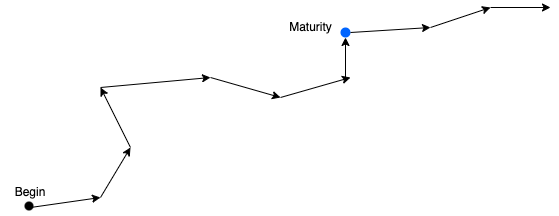
\includegraphics[scale=0.60,keepaspectratio=true]{images/02.png}
    \caption{Processo de consolidação do conhecimento}
    \label{knwledge_consolidation}
\end{figure}

Agora, mesmo que soubéssemos as melhores escolhas, de nada adiantaria chegar até aqui sem a correta manutenção de cada delas, ou seja, sendo que a cada nova decisão não fossem levadas em consideração todas as demais.

\begin{figure}[H]
    \centering
    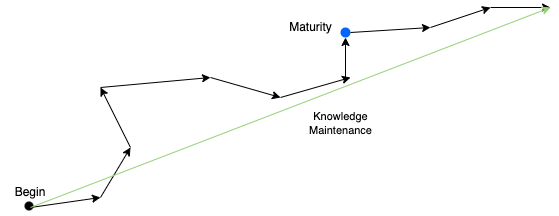
\includegraphics[scale=0.60,keepaspectratio=true]{images/03.png}
    \caption{Processo de manutenção do conhecimento}
    \label{knowledge_maintenance}
\end{figure}

Neste momento, estaríamos no que chamamos de ``Estado da Arte'' onde diversos setores da empresa poderia trabalhar munidos de manuais para execução de seus trabalhos, deixando a parte criativa a ser utilizada no momento da concepção de cada projeto. 

Mas se isso parece ser tão interessante, por quê nao se faz?

\section{Time em que está ganhando não se mexe?}

Acredito que uma das respostas mais óbvias é a de que ``time em que está ganhando não se mexe’’. Mas dai vai outra pergunta: e se Messi, Neymar, Cristiano Ronaldo tivessem iniciado a carreira em um time que estivesse ganhando, o que seriam deles?. Qualquer processo deve ser analisado quantas vezes forem necessários pois 1) você consegue melhorar o processo OU 2) você melhora a percepção que você tem do processo. Ou seja, sempre há uma melhora.

Não digo que a Hotmart nunca tenha feito mudanças nos códigos, mas clamo para que algum verdadeiramente profundo seja feito.

\section{O Monte Everest}

Outra frase muito ouvida é de que esse processo ou aquela informação é utilizada por tanta gente que me parece ser mais fácil Escalar o Monte Everest do que propor alguma mudança em meu contexto de trabalho.

\section{A Inovação}

Uma vez em que estivermos rodando os nossos trabalhos no ``Estado de arte'', sobrará muito tempo livro para criarmos e inovamos. 

Por exemplo, imagine se a Hotmart fosse da seguinte maneira:
\begin{figure}[H]
    \centering
    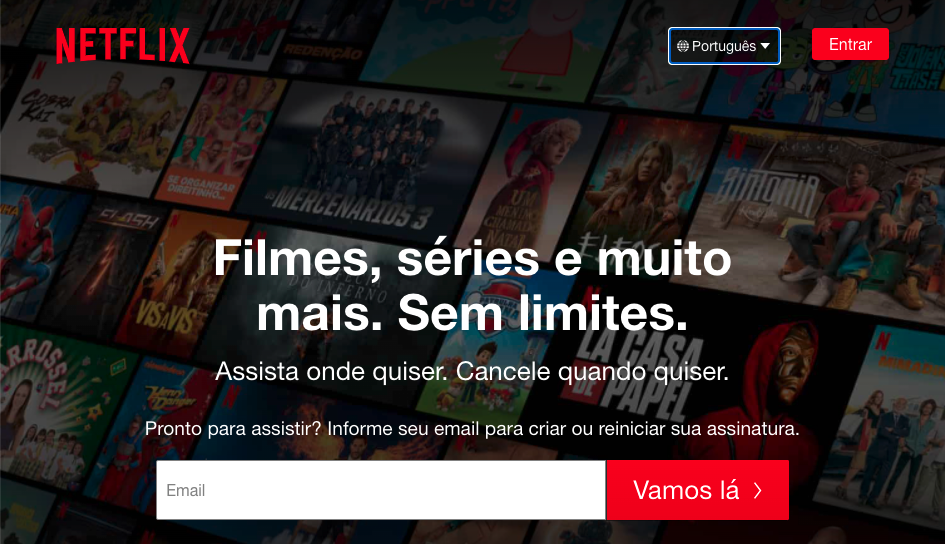
\includegraphics[scale=0.37,keepaspectratio=true]{images/04.png}
    \caption{Tela de login independente de haver compras}
\end{figure}

\begin{figure}[H]
    \centering
    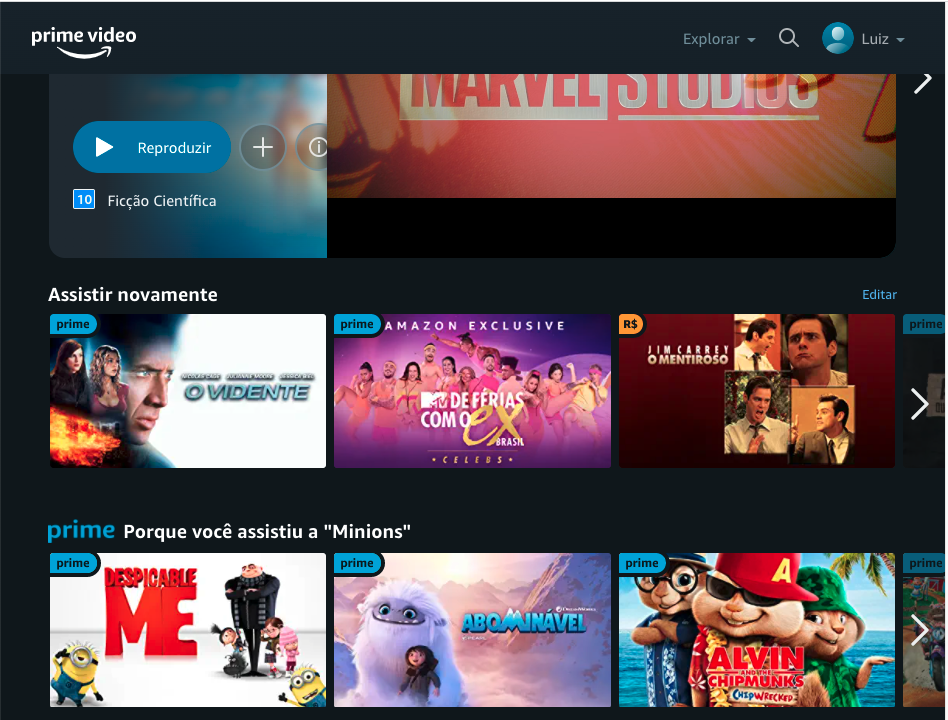
\includegraphics[scale=0.30,keepaspectratio=true]{images/05.png}
    \caption{Novidades do catálogo Hotmart, conteúdo gratuito oferecido pelo produtor como um trailer de seu produto}
\end{figure}

\begin{figure}[H]
    \centering
    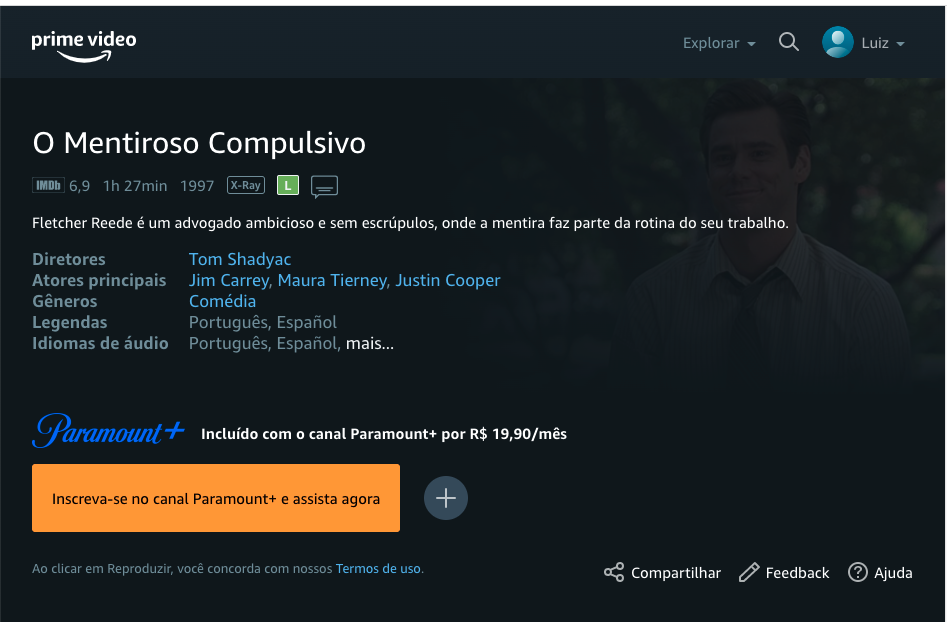
\includegraphics[scale=0.40,keepaspectratio=true]{images/06.png}
    \caption{Página de vendas de um pequeno, médio ou grande produtor}
\end{figure}

\begin{figure}[H]
    \centering
    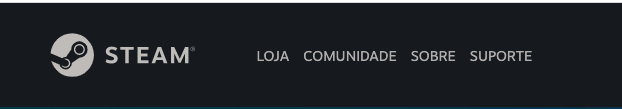
\includegraphics[scale=0.50,keepaspectratio=true]{images/07.png}
    \caption{Tela superior deve conter: COMPRAR - MINHAS COMPRAS - VENDER - MINHAS VENDAS - AJUDA}
\end{figure}

\section{Conclusão}

Acredita-se que se a plataforma por voltada para o comprador, conseguiremos melhores performances justamente pelo efeito orgânico da internet. A ideia é posicionar a Plataforma onde YouTube, Amazon Prime e Netflix não posicionaram. Seria ficar ali no meio deles servindo o que eles não servem. 

Imagine ver aquela gameplay completinha do seu gamer favorito pagando 3,99 sem anúncio? e ainda ter uma porrada de funcionalidade exclusiva. Seria muito melhor, pelo menos eu acho. E eles têm muitas dores com o YouTube onde sao cancelados por direitos autorais. Na nossa plataforma, ele poderia colocar uma música do Pink Floyd se quisesse desde que recolhesse os direitos aos autores. Seria um modelo onde todo mundo ganha.

Poderíamos aplicar o reembolso que nem na Steam: jogou por mais de 2 horas, sem reembolso. Isso iria reduzir bastante demanda de suporte e ticket pra gente. 

Fora que poderíamos fazer parcerias com as universidades para aprimorar nossos algoritmos de classificação, clusterização e sistema de busca e recomendação. 

\end{document}